\documentclass[fleqn,11pt,a4paper,dvipdfmx]{jsarticle}
%
\usepackage{amsmath,amssymb}
\usepackage{bm}
\usepackage[dvipdfmx]{graphicx}
\usepackage{bmpsize}  % ← バウンディングボックス用
\usepackage{ascmac}
\usepackage{multicol} 
\usepackage{paracol}
\usepackage{tikz}
\usepackage{caption}
\captionsetup[table]{justification=centering}
\captionsetup[figure]{justification=centering}
\usetikzlibrary{calc}
%
% \setlength{\textwidth}{\fullwidth}
% \setlength{\textheight}{39\baselineskip}
% \addtolength{\textheight}{\topskip}
% \setlength{\voffset}{-0.5in}
% \setlength{\headsep}{0.3in}
% \setlength{\mathindent}{0pt}  % 数式の左端インデントを0に
\vspace*{-\baselineskip} % ← 不要な最初の空白を詰める
\usepackage[
  left=2cm,    % 左だけ広め
  right=2cm,   % 右は狭め
  top=2cm,     % 上も狭め
  bottom=1.5cm   % 下も狭め
]{geometry}
%
\newcommand{\divergence}{\mathrm{div}\,}  %ダイバージェンス
\newcommand{\grad}{\mathrm{grad}\,}  %グラディエント
\newcommand{\rot}{\mathrm{rot}\,}  %ローテーション
%
% \pagestyle{myheadings}
\begin{document}
%
%
1 AEI 3番 : 馬場 悠斗
\setcounter{section}{2} 
\section{直並列R-L-C回路の瞬時関係}


ここでは、より一般的な2端子受動回路を取り上げ、配電と無効成分間のエネルギー交換に関連する典型的な特性を示す。
図3.5は、直列R-C分岐によって分流された直列R-L分岐を持つR-L-C回路である。
この形式の回路が特に興味深いのは、Hallenが報告しているように、抵抗R1,R2のエネルギー散逸の瞬間的な割合を時間不変にすることができるからである。
図3.5の回路方程式は、理想的な正弦波電圧供給で、

\begin{center}
  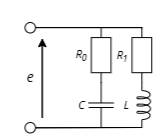
\includegraphics[width=0.3\linewidth]{./Circuits/Circuits_Z3_5.png}
  \captionsetup{labelformat=empty} % ← 番号を出さない設定
  \captionof{figure}{図3.5 回路の構成例}
\end{center}

\setcounter{section}{4} 
\section{正弦波電源電圧を用いた非線形回路}

家庭用電力定格における非線形負荷の使用は,1970年代に大幅に増加した.
テレビ受信機やラジオ受信機,調光器,多段変速電動機器などの機器には,通常,制御整流素子または非制御整流素子が組み込まれている.
テレビ受信機には入力整流器が備わっており,電源電流には直流成分が含まる.
図5.1に示すモノクロテレビの典型的な電源電流オシログラムは,波形の半波特性を示している.

\begin{center}
  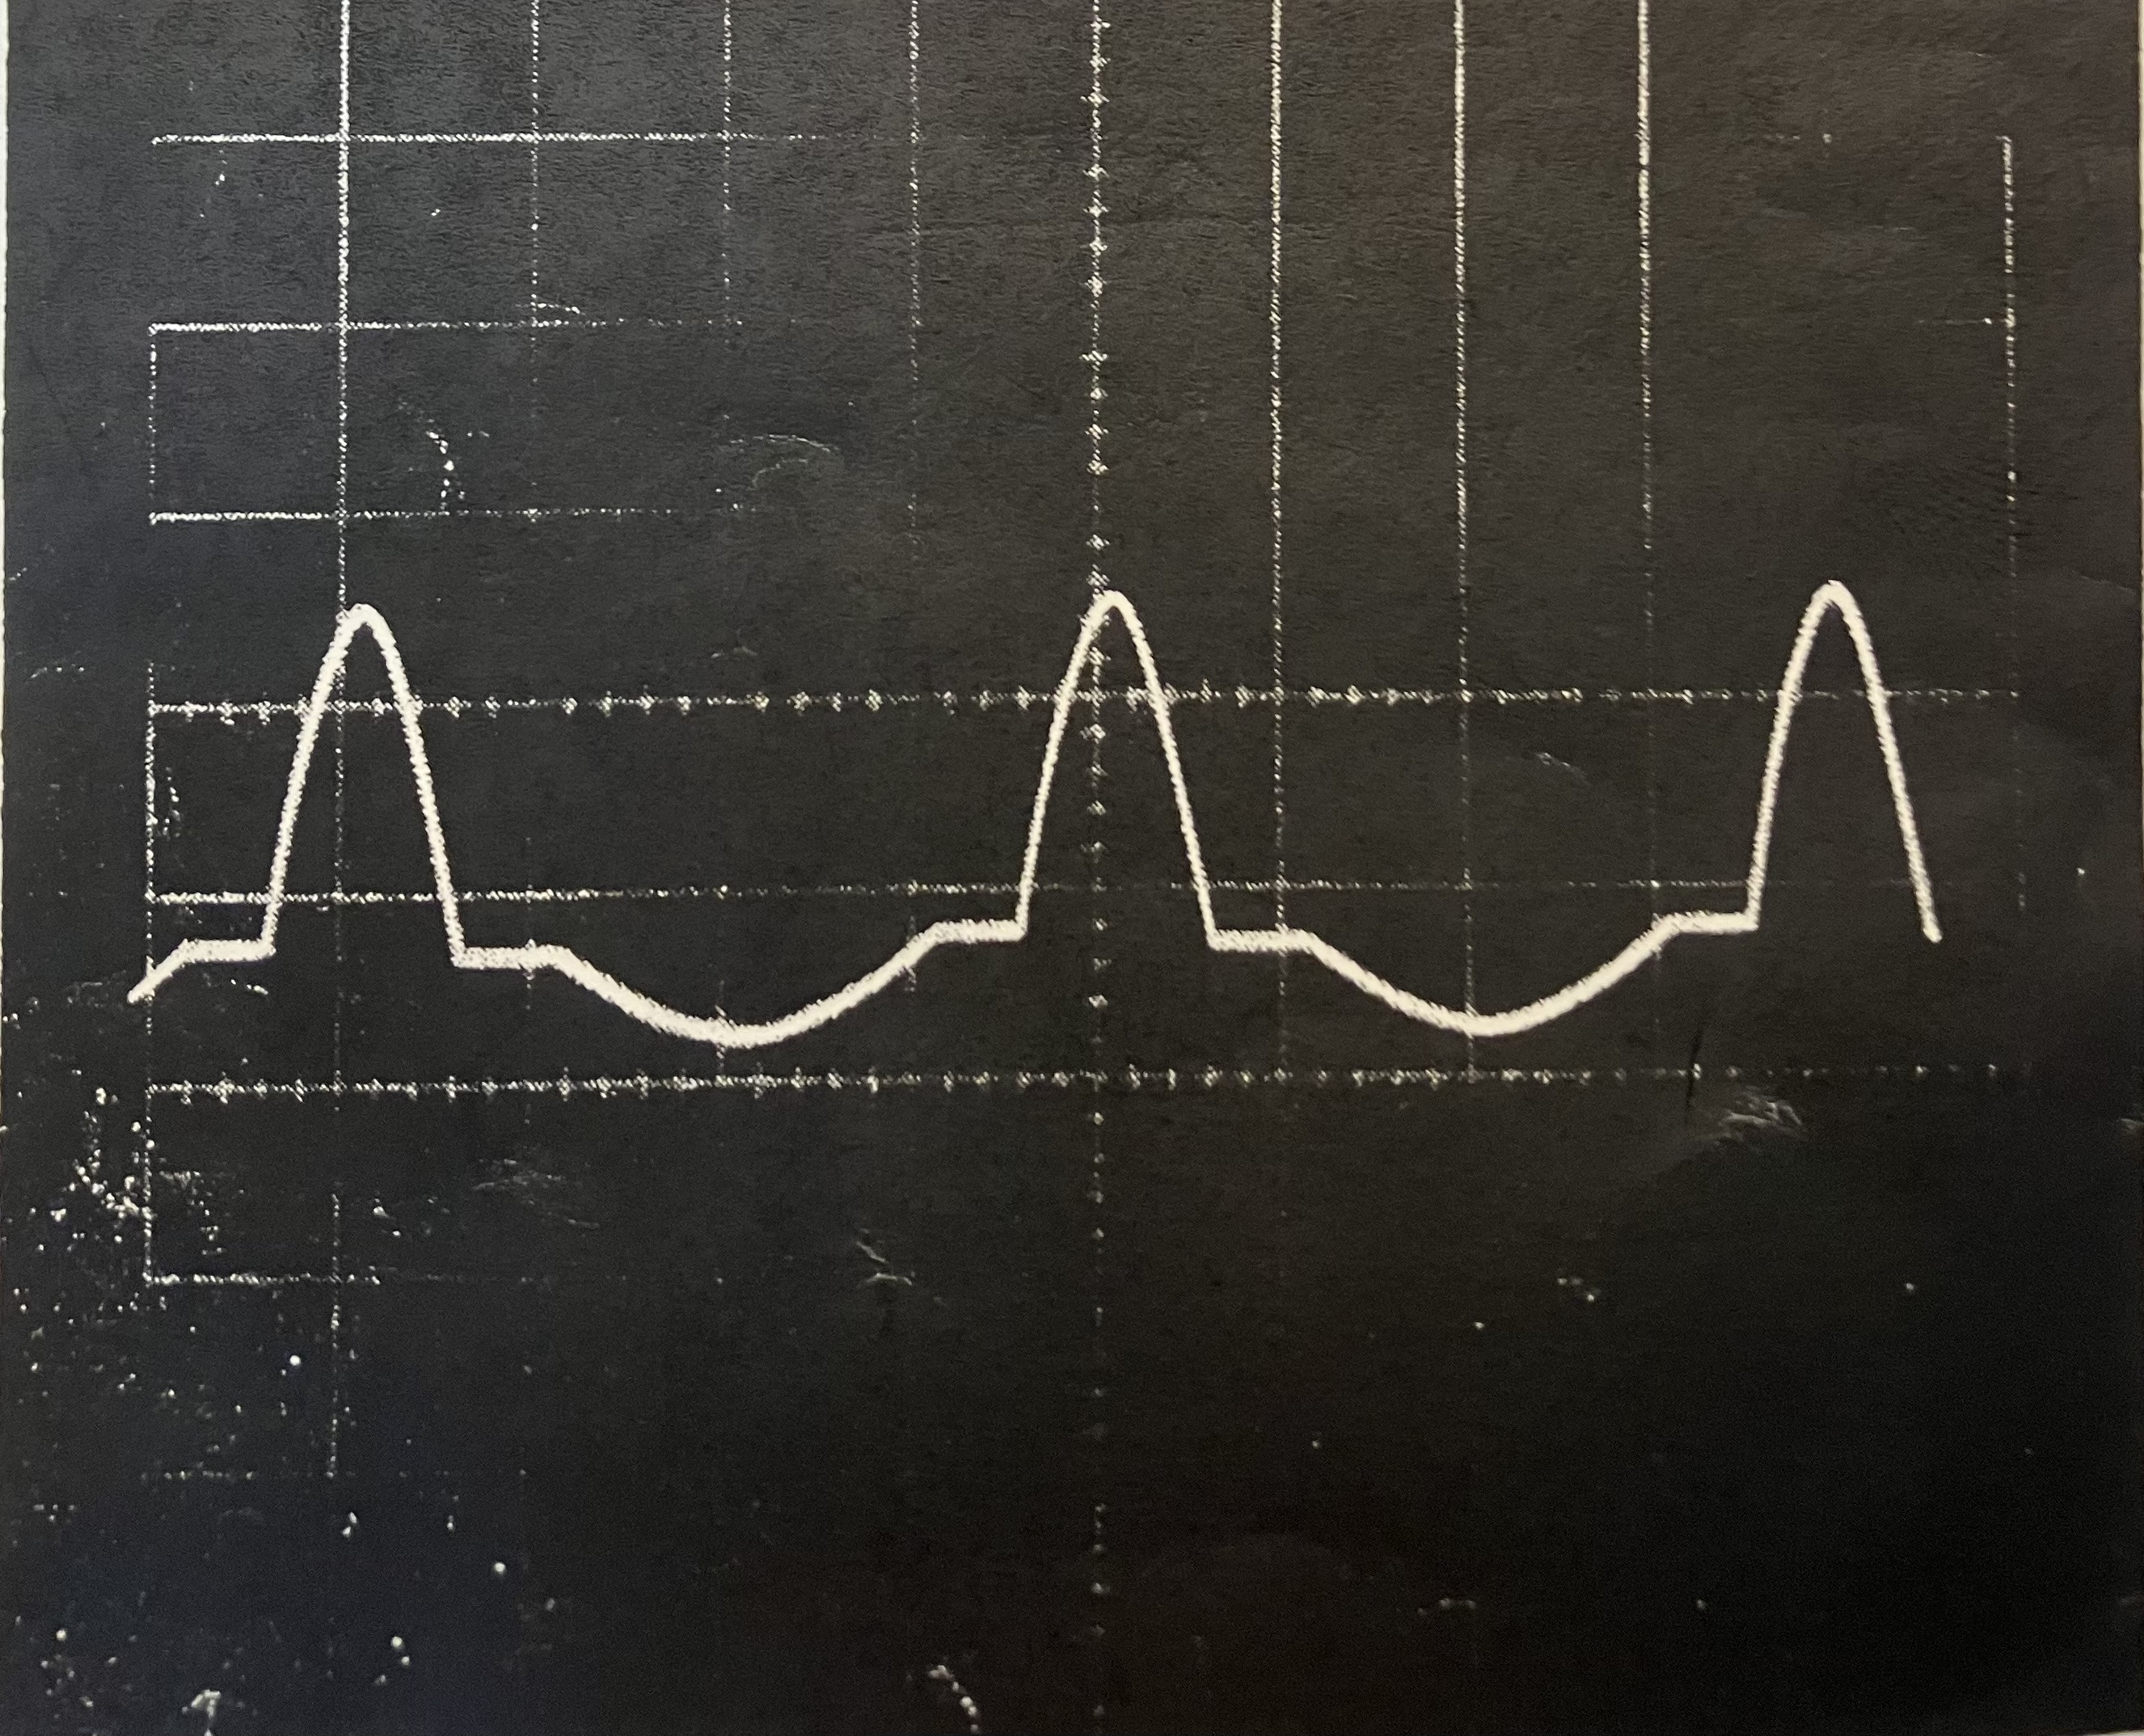
\includegraphics[width=0.3\linewidth]{./Circuits/fig5_1.jpg}
  \captionsetup{labelformat=empty} % ← 番号を出さない設定
  \captionof{figure}{図5.1 モノクロテレビ受信機の電源電流波形}
\end{center}

これには,9次高調波までの大きな高調波電流と直流電流項(図5.2)が含まれてる.
\begin{center}
  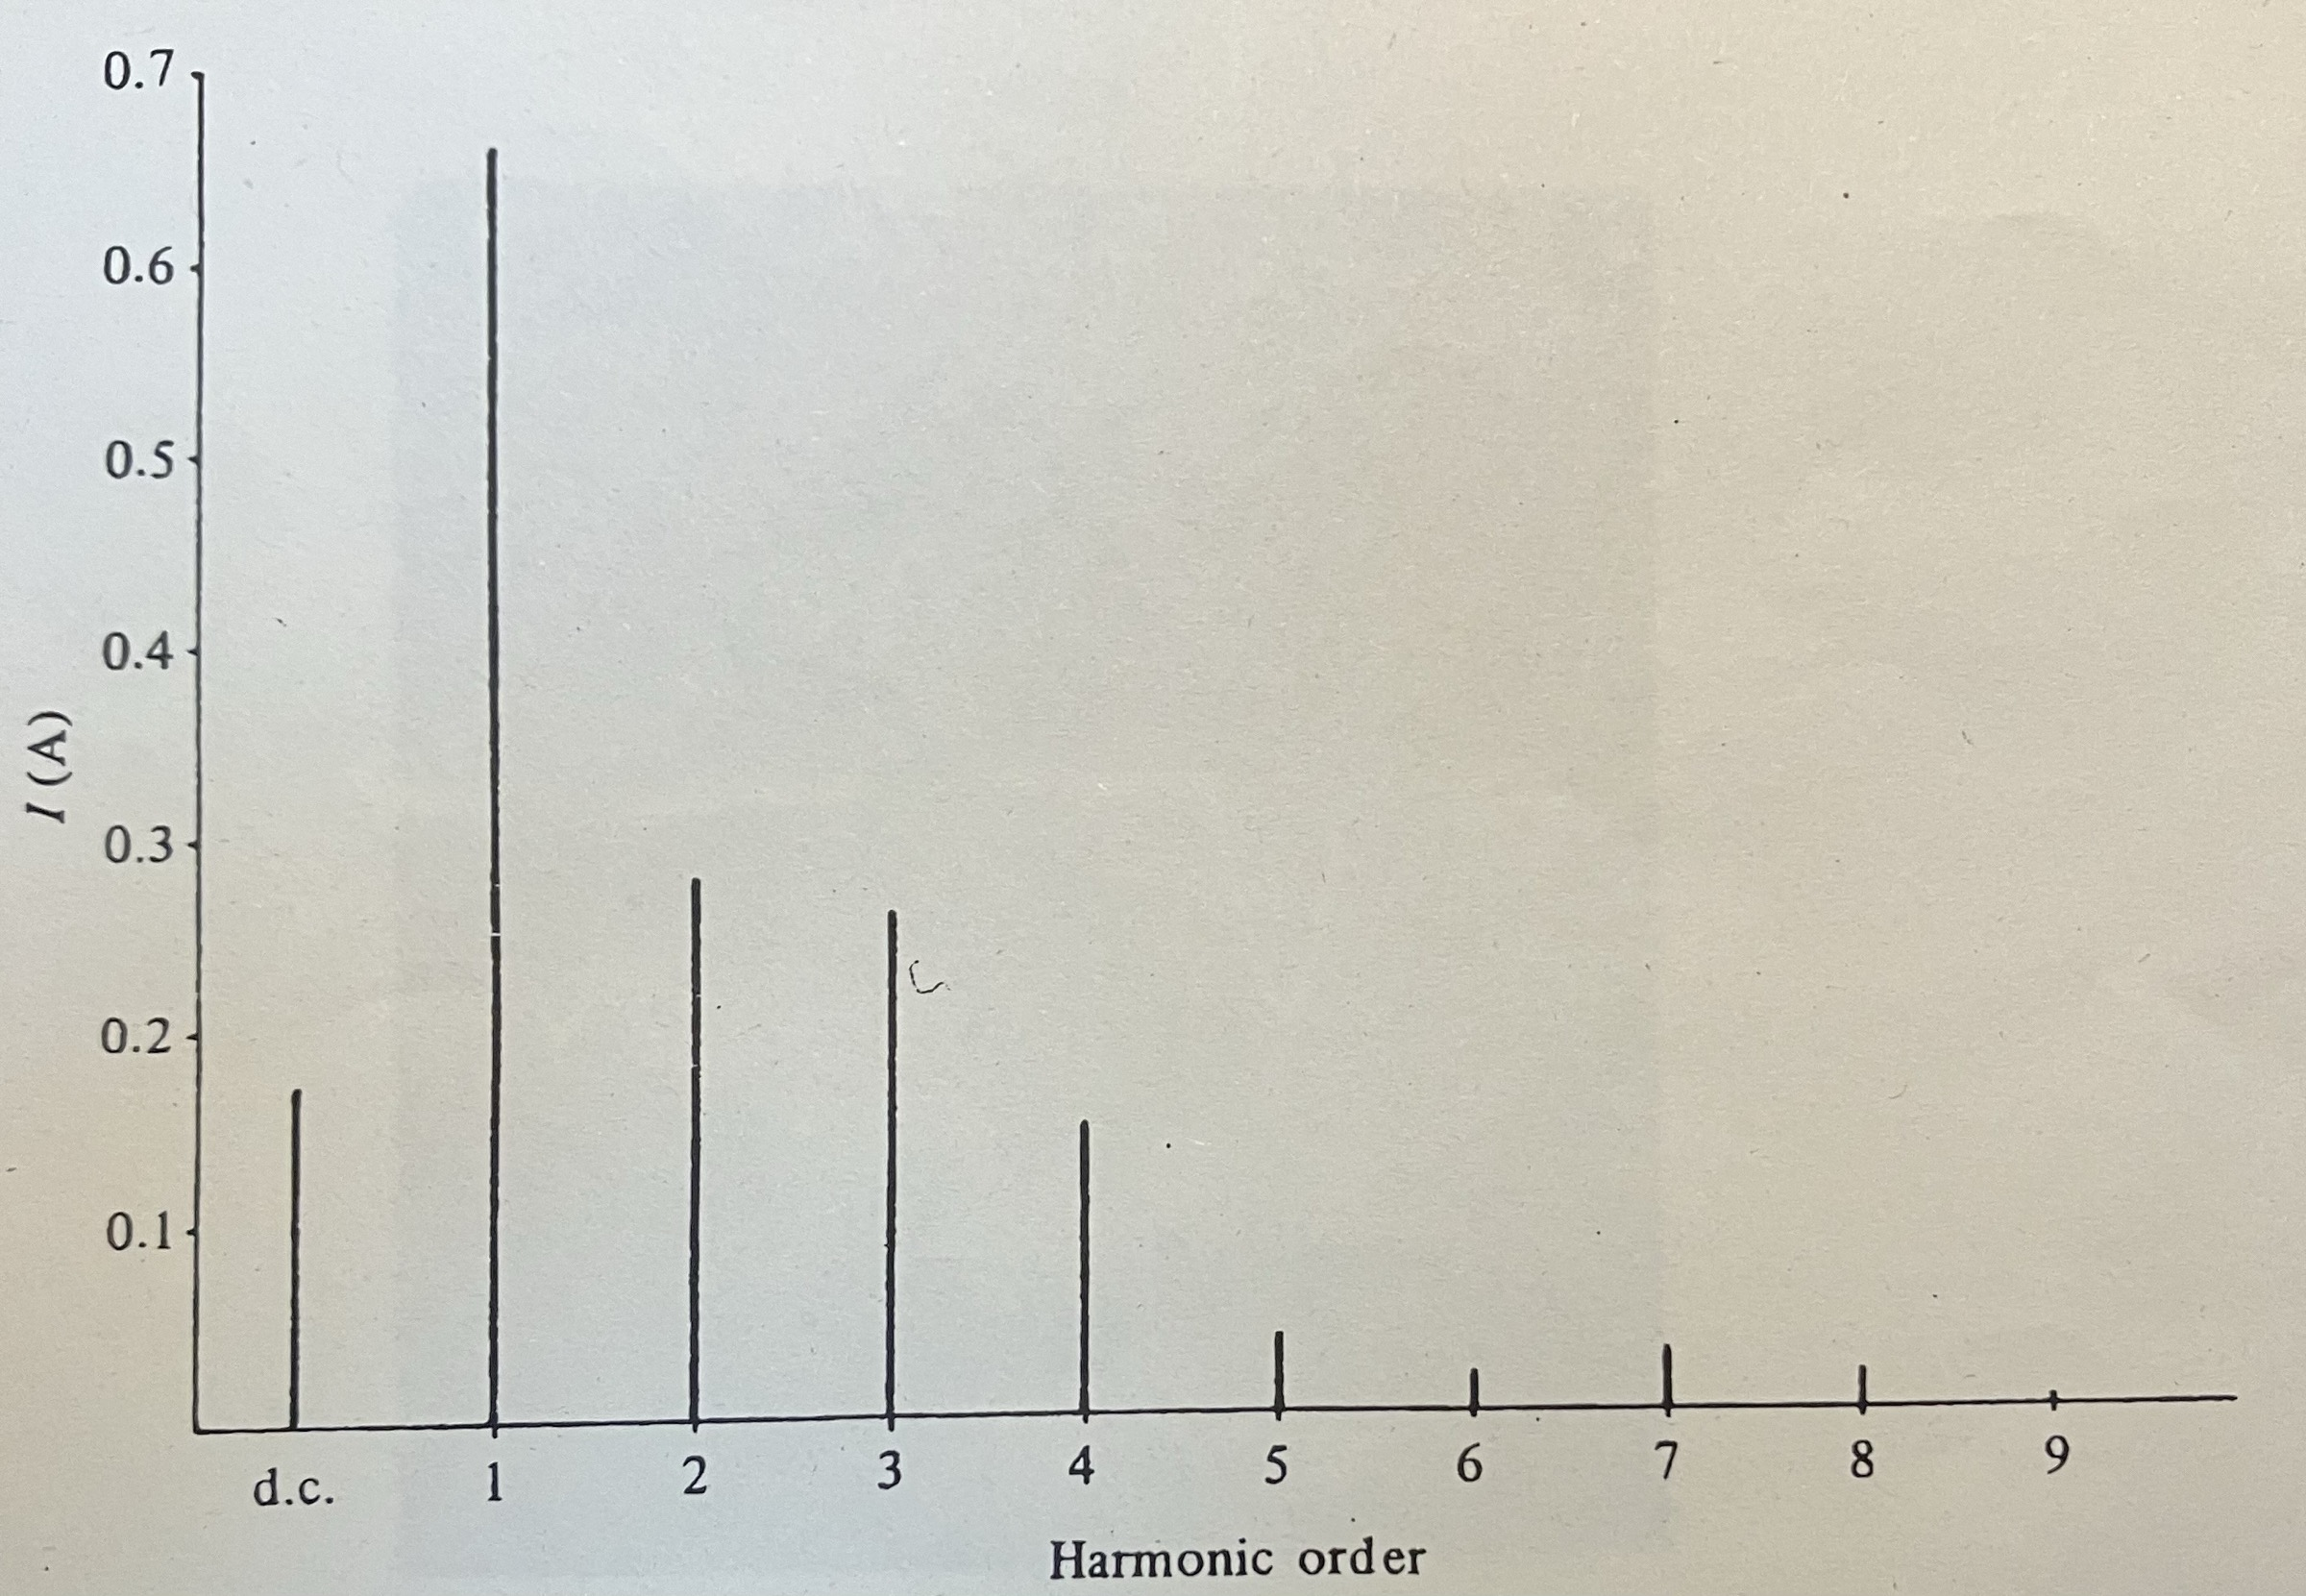
\includegraphics[width=0.3\linewidth]{./Circuits/fig5_2.jpg}
  \captionsetup{labelformat=empty} % ← 番号を出さない設定
  \captionof{figure}{ 図5.2 図5.1の供給電流波形の高調波成分}
\end{center}

英国製の標準的な21インチカラー受信機では,図5.3の波形が測定され,50Hzのスパイクのピーク値は7Aである.
\newpage
\begin{center}
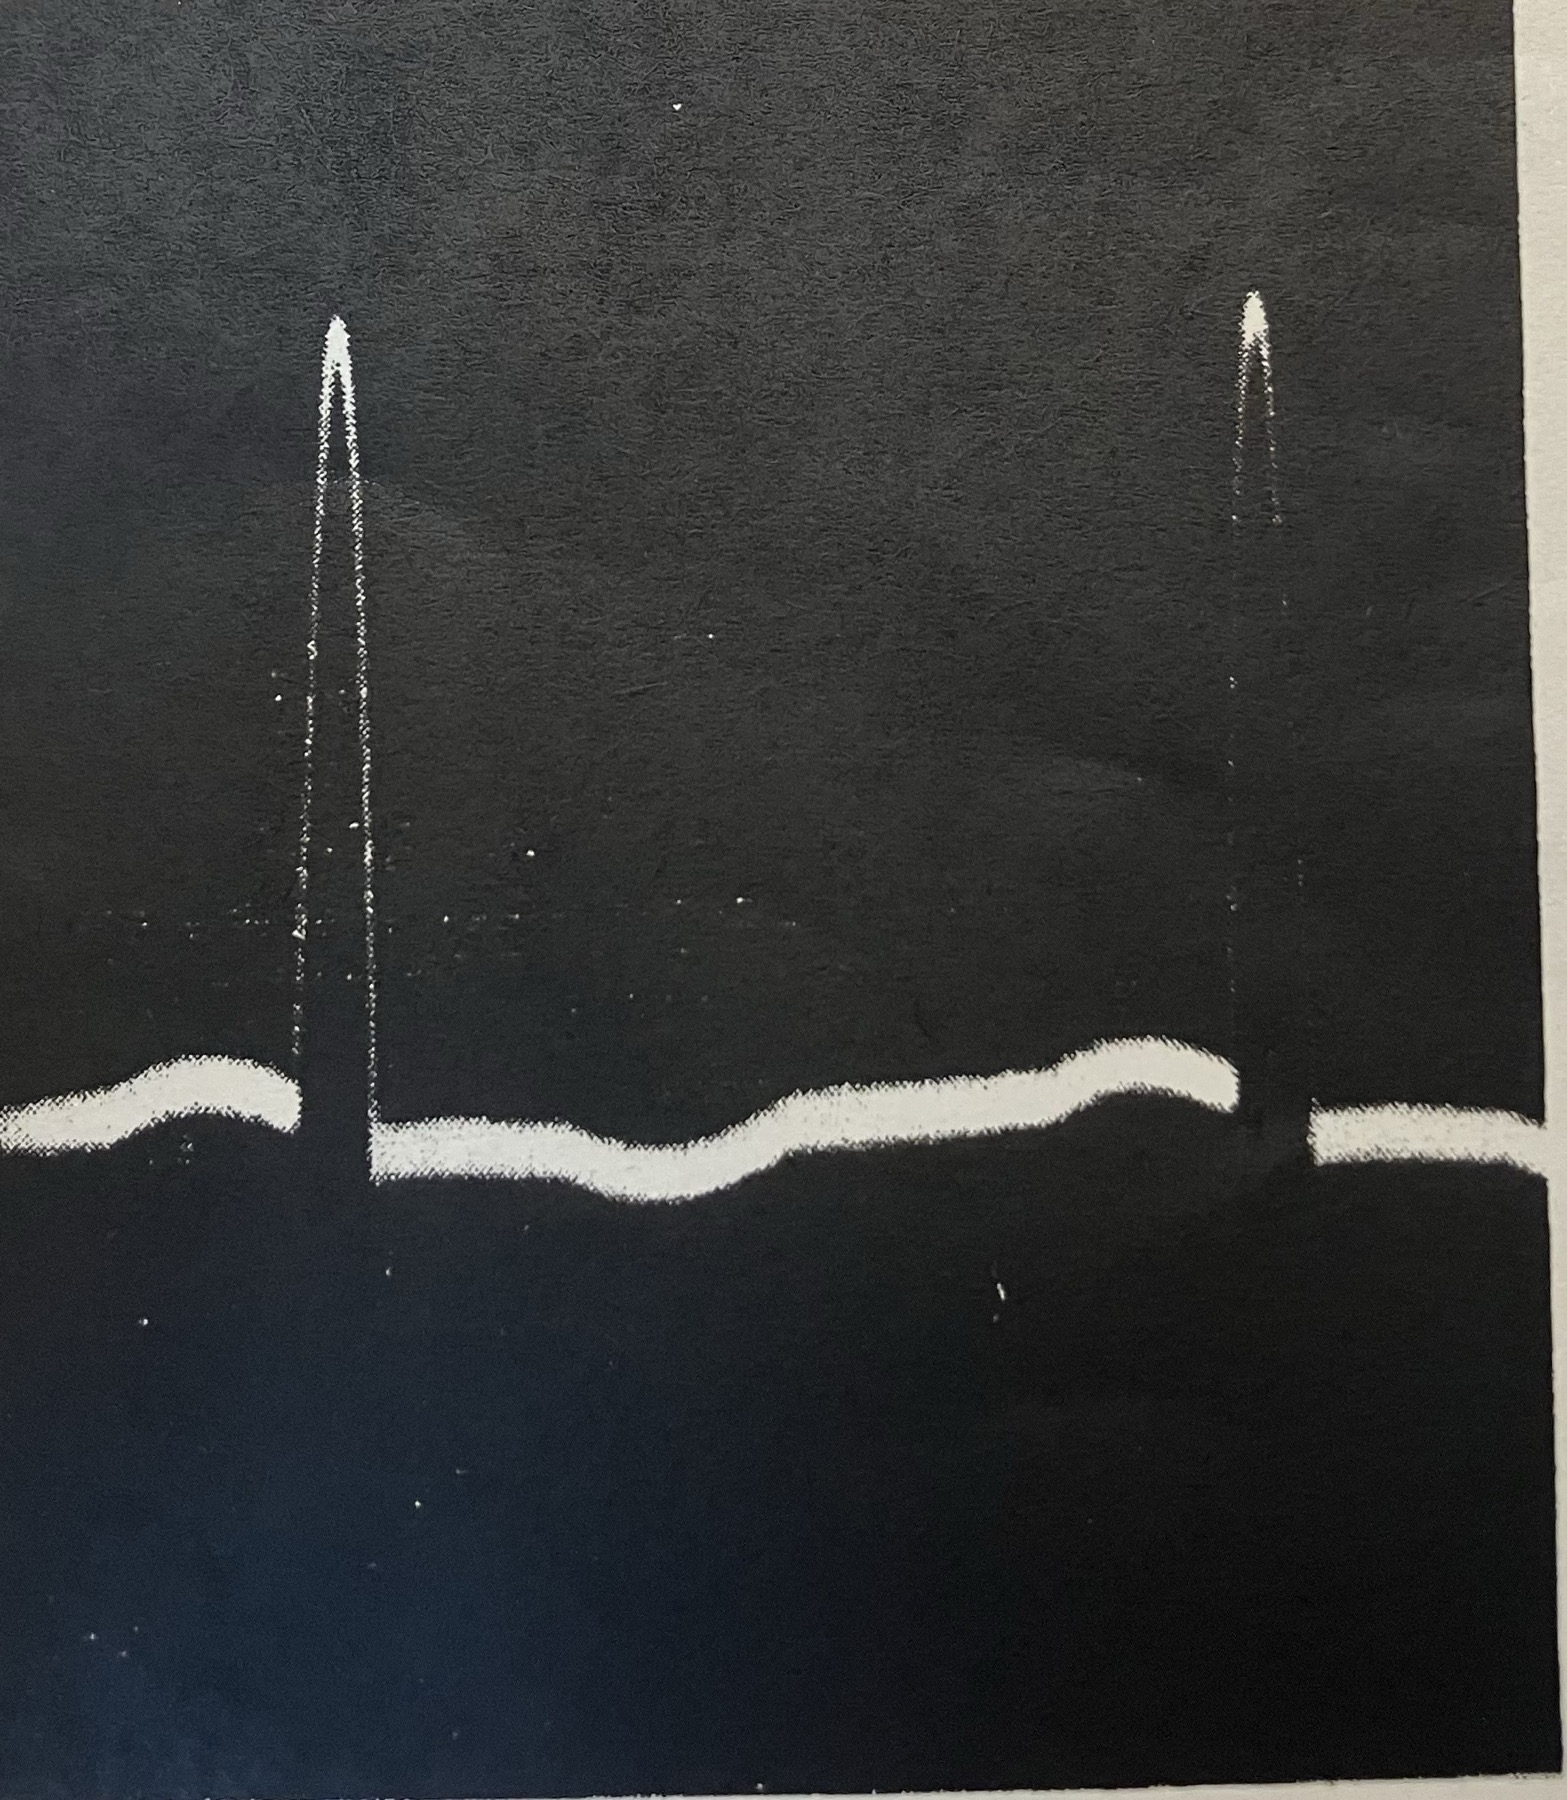
\includegraphics[width=0.3\linewidth]{./Circuits/fig5_3.jpg}
\captionsetup{labelformat=empty} % ← 番号を出さない設定
\captionof{figure}{図5.3 英国製21インチカラーテレビ受信機の電源電流波形\newline スパイク電流=50Hzでピーク7A}
\end{center}

最近のカラー受信機では,電源ラインから直流電流を除去するために,電源に全波整流器の入力段が装備されている.
典型的な電源電流波形を図5.4のオシログラムに示す.
\begin{center}
  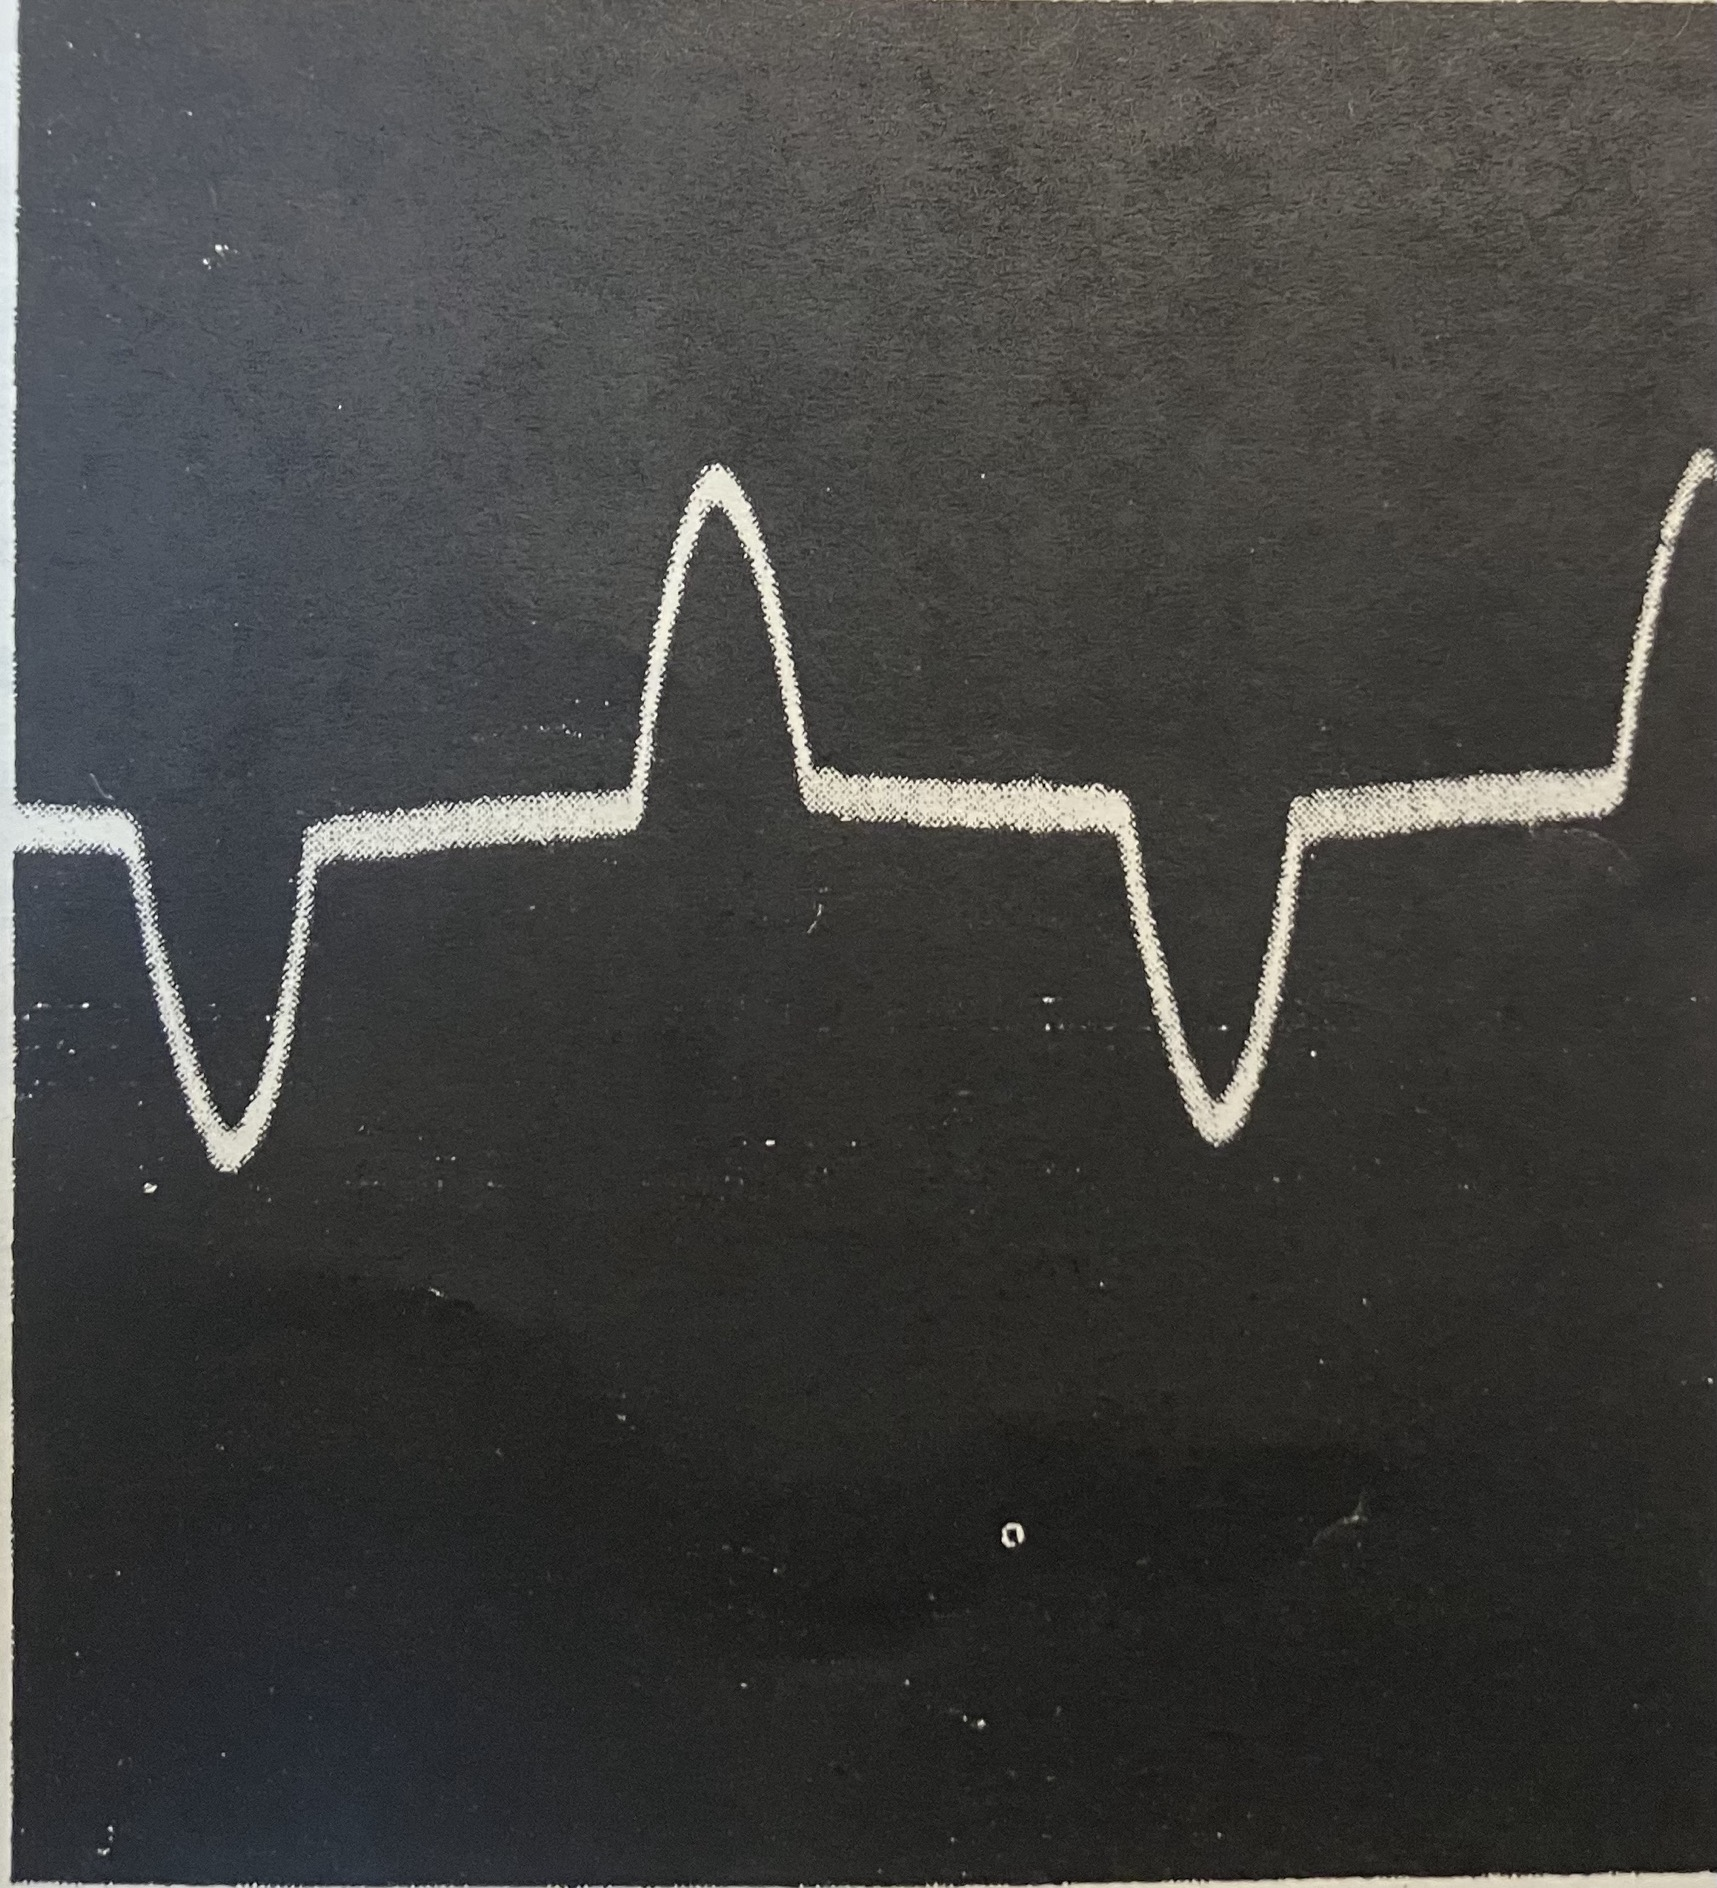
\includegraphics[width=0.3\linewidth]{./Circuits/fig5_4.jpg}
  \captionsetup{labelformat=empty} % ← 番号を出さない設定
  \captionof{figure}{図5.4 全波整流入力段を備えたカラーテレビ受信機の電源電流波形}
\end{center}
例えば1976年には,英国には1,800万台のテレビ受信機があり,そのうち約半数がカラー受信機であった.

電気アーク炉やサイリスタ制御モーターなどの産業用負荷は,配電系統に大きな非線形インピーダンスを生じさせる.
例えば,アーク炉の負荷サイクルの最初の部分(3~8時間)は溶融期間と呼ばれ,固体装入物が溶融する.
この期間は,アークの不安定性とスクラップ金属の移動によって引き起こされる激しい電流変動が特徴である.
これらの電流変動は不規則で正確に予測することは不可能であり,供給システムのインピーダンスにおける電流の変動により,
他の電力消費機器への供給電圧の低下を引き起こす可能性がある.
しかしながら,非線形回路におけるエネルギーの流れと電力分配を研究するためには,
電源から非正弦波の電流が流れているにもかかわらず,供給電圧がほぼ正弦波のままであるアプリケーション群を区別することが有用である.
このようなシステムは,エネルギーの観点から興味深い特性を持つことが分かっており,これらの特性は力率改善の可能性のある方法について有用な知見をもたらす.
%
%
\end{document}